%\documentclass[%
%reprint,
%%singlecolumn,
%superscriptaddress,
%%groupedaddress,
%%unsortedaddress,
%%runinaddress,
%%frontmatterverbose, 
%%preprint,
%%showpacs,preprintnumbers,
%%nofootinbib,
%%nobibnotes,
%%bibnotes,
%%pre, 
%floatfix,
%amsmath,
%amssymb,
%aps,
%notitlepage
%]{revtex4-1}
\documentclass[12pt]{article}
\usepackage{amsmath}
\usepackage{amsfonts}
\usepackage{amssymb,graphicx,fullpage}
\usepackage{mathrsfs}
\usepackage{bm}
\usepackage[hidelinks=true]{hyperref} 
\usepackage{xcolor}
\usepackage{algorithm2e}
\usepackage{mathrsfs}
\usepackage{bm, amsbsy}
% `\NoCaptionOfAlgo'
\usepackage{tcolorbox}

\usepackage[hidelinks=true]{hyperref}
\usepackage{xcolor}
%\definecolor{greenish}{rgb}{0.13,0.58,0.16}
\definecolor{greenish}{RGB}{141,198,63}
\definecolor{reddish}{RGB}{239,65,54}
\definecolor{blueish}{RGB}{28,117,188}
\definecolor{alg1}{RGB}{122,89,239}
\definecolor{alg2}{RGB}{245,147,106}
\definecolor{alg3}{RGB}{124,198,137}

\hypersetup{
colorlinks   = true, %Colours links instead of ugly boxes
urlcolor     = blueish, %Colour for external hyperlinks
linkcolor    = reddish, %Colour of internal links
citecolor   = greenish %Colour of citations
}

\def\grad{\nabla}
\def\at{\hat{a}}
\def\Ai{\mathcal{A}}
\def\H{\mathcal{H}}
\def\J{\mathcal{J}}
\def\R{\mathbb{R}}
\def\d{\text{d}}
\def\e{\text{e}}
\def\r{\mathbf{r}}
\def\x{\mathbf{x}}
\def\xst{\mathbf{x}^*}
\def\u{\mathbf{u}}
\def\a{\mathbf{a}}
\def\T{\mathsf{T}}
\def\R{\mathbb{R}}
\def\E{\mathbb{E}}
\def\S{\mathcal{S}}
\def\pol{\pi_\theta}
\def\qsa{Q (s, a)}
\def\paa{\pi(a, s)}
\def\H{\sigma}
\def\grad{\nabla}
\def\th{\hat{\mathbf{t}}}
\def\ph{\hat{\mathbf{p}}}
\def\nh{\hat{\mathbf{n}}}
\def\yd{\dot{y}}
\def\ite{\text{ite}}
\def\P{\mathcal{P}}
\def\D{\mathcal{D}}
\def\Z{\mathcal{Z}}
\def\ah{\hat{a}}
\def\theta{\vartheta}
\DeclareMathOperator*{\argmax}{arg\,max}

\newtcolorbox{myalgorithm}[2][]{%
    fonttitle=\bfseries,
    title=#2,
    #1,
    before upper={\begin{algorithm}[H]},
    after upper={\end{algorithm}}
}

\begin{document}
% \title{Influence of innate behavior on the dynamics of innovation in foraging}
\title{Dynamics of innovation along foraged trajectories}
\author{S Ganga Prasath}
%\email{sgangaprasath@iitm.ac.in}
%\affiliation{Department of Applied Mechanics, Indian Institute of Technology Madras, Chennai TN 632406.}
\date{}

%\begin{abstract}
%For later...
%\end{abstract}

%\pacs{Valid PACS appear here}
\maketitle
\section{2D grid world}
Let us say an agent has an intrinsic behavior to follow a herd or a trail
laid by other ants or a flock of birds. All the agents simply following this
herd following behavior will not result in new solutions. Agents often have
to innovate and find new solutions either because the trails are not available
anymore or because you know a better route (influence of history) or perturbations
(intrinsic or environmental) can throw you off trails and you have to find new solutions.
We are interested in understanding the role of intrinsic behavior on the dynamics of innovation.

We will start by implementing an agent trying to optimally traverse from point
A to point B in a 2D grid world. The steps involved in traditional reinforcement
learning based on SARSA algorithm involves essentially 2-steps: $(i)$ action-value
function update, $(ii)$ policy update. The action-value update equation in on-policy SARSA is given by
\begin{align}
Q_\pi(s_t, a_t) \leftarrow & \ Q_\pi(s_t, a_t) \nonumber \\
& \ + \alpha \{ r_{t+1} + \gamma Q_\pi(s_{t+1}, a_{t+1}) - Q_\pi(s_t, a_t) \}
\end{align}
while the policy update is given by
\[
\pi(s) = \argmax_a Q(s, a).
\]
This is shown in algorithmic form in Alg.~\ref{alg:rlsealg}. \\[5pt]

\begin{center}
\begin{tcolorbox}[colframe=alg1!50,colback=alg1!10,fonttitle=\bfseries, title=Algorithm~\ref*{alg:rlsealg}: SARSA algorithm for action-value update]
\begin{algorithm}[H]
\textit{Initialize}:
State, $s_0$;
action, $a_0$;
action-value function, $Q(s_j, a_j)$

\ForEach{epoch}{
Update action-value function using SARSA rule:
    \begin{align*}
    	Q_\pi(s_t, a_t) \leftarrow & \ Q_\pi(s_t, a_t) + \alpha \{ r_{t+1} + \gamma Q_\pi(s_{t+1}, a_{t+1}) - Q_\pi(s_t, a_t) \}
    \end{align*}
 Choose action:
 \begin{align*}
 \pi(s_t) =& \ \argmax_a Q(s_t, a_t)
 \end{align*}
 Calculate reward, $r_t$
 
 Check if target $s^*$ is reached, continue if not
}
\caption[Recursive least-squares estimator: $\pi \approx \pi^*$]{}\label{alg:rlsealg}
\end{algorithm}
\end{tcolorbox}
\end{center}

\section{Trail following behavior}
Consider a trail of pheromone $\x^*(s)$ represented by arc-length parameterization $s$.
The concentration field in 2D is then given by $c(\x) = c_o \delta(\x-\x^*(s))$.
This filed of course is assumed to be steady but can be made time-dependent by simply adding a decay time-scale $\tau$ to get: $c(\x, t) = c_o \delta(\x-\x^*(s)) \e^{-t/\tau}$. We can immediately evaluate some of the properties of the curve $\x^*(s)$ which will come in handy soon: $\th(s) = \d \x^*(s)/\d s = \{ \cos \psi(s), \sin \psi(s) \}$ and $\nh(s) = \{ \sin \psi(s), \cos \psi(s) \}$. As we can see the entire curve $\x ^*(s)$ can be represented only using $\psi(s)$ up to global translations and rotations, which is a well known property of curves in 2D.

The state of the agent/ant in our problem is represented by its coordinates
$\r(t)=\{ r_x(t), r_y(t) \}$ and it can make measurements about how far from the
pheromone trail it is $\d\r(t)$ as well as the orientation of the trail, $\th(s, t)$.
The action that it takes from these measurements is to align its orientation, $\ph(t)$
along a direction that will take it towards the trail. We show in Fig.~\ref{fig:schm1}
a schematic of the problem set up.The strategy used by the agent for tracking the pheromone
trail will be to move along the direction given by $(\d \r/|\d \r| + \th)$ by a fixed
length $h$. In order to identify the location along $\xst(s)$ where $\d \r$ intersects,
we use the condition $\d\r(t) \perp \th(s,t)$.

\begin{figure}
    \centering
    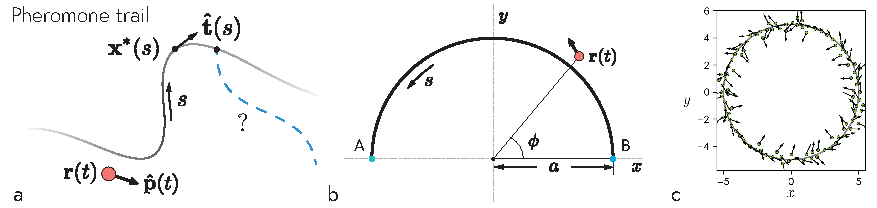
\includegraphics[width=\textwidth]{./figs/schematic.pdf}\label{fig:schm1}
    \caption{Schematic of setup}
\end{figure}

\subsection{Semi-circular trail}
For the problem at hand, we will considering a semi-circular trail whose coordinates can be
written in arc-length form as $\xst(s) = \{ a \cos(s/a), a \sin(s/a) \}$ where $a$ is the radius
of the circle. The trail starts at $s=0$ given by coordinates $\xst(0) = \{ a, 0 \}$ and ends at
$s=\pi a$ at $\xst (\pi a) = \{ -a, 0 \}$. From this it is easy to find that $\th(s) = \{ -\sin(s/a) , \cos(s/a) \}
= \{ \cos(\pi/2 + s/a), \sin(\pi/2 + s/a) \}$, and $\nh(s) = \{ -\cos(s/a) , \sin(s/a) \}$. We see that we
can represent $\th(s)$ through $\psi(s) = (\pi/2 + s/a)$. We can now calculate the location along the arc-length
where $\r(t)$ is closest by using the constraint condition $\d\r(t) \perp \th(s,t)$ or equivalently $\d\r(t)
\cdot \th(s,t) = 0$. We can now write $\d \r(t) \sim \{ a \cos(s/a) - r_x, a \sin(s/a) - r_y \}$
(up to normalization) and get the location $s_*(t) = a \tan^{-1}(r_y/r_x)$ by using the formula
for $\th(s)$. From this it is trivial to see that the angle along $\d \r$ is $\phi(t) = \tan^{-1}(r_y/r_x)$
(as is evident in Fig.~\ref{fig:schm1}$(b)$). For a given location of the agent, $\r(t)$ the orientation
it needs to take in the next step can be easily calculated to be $\theta(t) = (\pi/4 - \phi(t))$.

We can now set up the entire dynamics of the agent's trail following behavior on this semi-circle. We can state this
in the notation of reinforcement learning as it will become helpful later. The state of the agent
is $S^t = \{ r_x^t, r_y^t \}$, the measurements it makes are $M^t = \phi^t$ and using this information
the action the agent takes is $A^t = \{ \theta^t \}$ which is its orientation. The dynamics of
the agent can now be written as follows:
\begin{align}
    \text{Measurement update: } \phi^{t+1} = & \ \tan^{-1} \bigg( \frac{r_y^t}{r_x^t} \bigg) + \zeta^t, \\
    \text{Action update: }\ph^{t+1} =& \ \th^{t+1} + \d\r^{t+1}, \\
    \text{State update: } \r^{t+1} =& \ \r^t + l \ph^{t+1},
\end{align}
where $\r^t = \{ r_x^t, r_y^t \}$, $\d\r^t = (\xst(s^t)-\r^t)/||\xst(s^t)-\r(t)||$ and $\ph^t = \{ \cos \theta^t, \sin \theta^t \}$.
We have added sensory noise $\zeta^t$ (which is sampled from a uniform distribution) to the measurement
to reflect the error that accompanies measurements usually. The solution dynamics is shown
in Fig.~\ref{fig:schm1}$(c)$. We call this line-following behavior as a policy
$\pi_\ite(\r, \phi): $
which denotes the agent's innate behavior to follow pheromone trails.

\section{Ornstein-Uhlenbeck process}

Let us consider an agent whose orientation $\ph = ( \cos \theta, \sin \theta)$ wants to relax to a
neutral orientation with stochasticity associated with estimation error. The dynamics of the orientation
can be written as a stochastic differential equation given by
\begin{align}
    \dot{\theta}(t) =& \ - \alpha \theta(t) + \sqrt{2 D} \eta(t), \\
    \langle \eta(t) \eta(0) \rangle =& \ \delta(t).
\end{align}
This is the evolution of the famous Ornstein-Uhlenbeck process which has been extremely well studied
and the evolution of the probability density can be solved exactly. The Fokker-Plack equation for
its dynamics which provides the probability of a given state $\theta(t)$ i.e. $p(\theta, t)$, is given by
\[
    \frac{\partial p}{\partial t} = \alpha \frac{\partial(\theta p)}{\partial \theta }
    + D \frac{\partial^2 p}{\partial \theta^2}
\]
The dynamics of the angle relaxes to equilibrium angle $\theta = 0$ in the absence of fluctuations.
The evolution of the mean is $\dot{h}(t) = - \alpha h(t)$ where $h(t) = \langle \theta(t) \rangle$
while the co-variance dynamics is given by $\dot{\zeta}(t) = -2\alpha \zeta(t) + 2D$ with
$\zeta = \langle {(\theta(t) - h(t))}^2 \rangle = \langle \theta^2(t) \rangle - h{(t)}^2$.

The position of the agent evolves as $\dot{\r}(t) = v_o \ph(t)$. Under the assumption that the angle
is small, we can write $\dot{\r}(t) = v_o (1, \theta)$. Thus we have $\yd (t) = v_o \theta$ which can
be used to rewrite the orientation equation as
\begin{align}
    \ddot{y}(t) =& \ - \alpha \yd (t) + v_o\sqrt{2 D} \eta(t).
\end{align}
This second order equation needs to boundary condition. We require $y(0) = 0$ and $\yd (0) = 0$ which
comes from setting the initial orientation to be 0. We are interested in the evolution of the mean and the variance of this SDE. Let $m(t)= \langle y(t) \rangle$
where the averaging is the ensemble average (equivalently the average of the several trajectories of the
same dynamics). The mean $m(t)$ evolves as
\begin{align}
    \ddot{m}(t) =& \ -\alpha \dot{m}(t).
\end{align}
By applying the above boundary condition, we can immediately see that $m(t) = 0$. Nevertheless, we are
interested in the evolution of the standard deviation, $\beta(t) = \langle {[y(t) - m(t)]}^2 \rangle$.
In order to derive an expression for that, we differentiate the definition once to get
\begin{align*}
    \dot{\beta}(t) =& \ 2 \langle \{ y(t) - m(t) \} \{ \yd(t) - \dot{m}(t) \} \rangle, \\
    = & \ 2 \langle y \yd \rangle - 2 m \dot{m}, \\
    = & \ 2 v_o [ \langle y \theta \rangle - m \dot{m}].
\end{align*}
We can estimate $\langle y \theta \rangle$ as follows
\begin{align*}
    \langle y \theta \rangle =& \ v_o \E \bigg[ \int_0^t \theta(s) \theta(t) \ \d s \bigg], \\
    =& \ v_o  \int_0^t \langle\theta(t) \theta(s)\rangle \ \d s.
\end{align*}
We know that for an OU process, 
\[
\langle\theta(t) \theta(s)\rangle = \frac{D}{\alpha} \bigg[ \e^{-\alpha(t-s)}-\e^{-\alpha(t+s)} \bigg].
\]
From this we see that
\begin{align*}
    \langle y \theta \rangle =& \ \frac{v_o D}{\alpha} \int_0^t  \bigg[ \e^{-\alpha(t-s)}-\e^{-\alpha(t+s)} \bigg] \ \d s, \\
    =& \ \frac{v_o D}{\alpha^2} \bigg[ 1 - 2 \e^{-\alpha t} + \e^{-2 \alpha t}\bigg].
\end{align*}
We thus have the evolution of the co-variance of $y(t)$ as
\begin{align}
    \dot{\beta}(t) = & \  \frac{2 v_o^2 D}{\alpha^2} \bigg[ 1 - 2 \e^{-\alpha t} + \e^{-2 \alpha t}\bigg].
\end{align}
We finally have the variance as a function of time as
\begin{align}
    \beta(t) & = \frac{v_o^2 D}{\alpha^3} \bigg[ 2 \alpha t - \e^{-2 \alpha t} + 4 \e^{-\alpha t} - 3 \bigg].
\end{align}
For $t \gg \alpha^{-1}$ we can immediately see that $\beta(t) \approx 2v_o^2 D t/\alpha^2$. We are interested
in the variance at time, $t^* = c/v_o$ where $c$ is the distance of the agent from the goal A and $v_o$
is the intrinsic speed of the agent. At this time the location of the agent along x-axis is $x(t^*)=c$
while the variance in $y(t)$ is $\beta(t^*) \approx 2v_o D c/\alpha^2$.
% Differentiating this once more, we get
% \begin{align*}
%     \ddot{\beta}(t) =& \ 2 [ v_o \langle (\yd \theta + y \dot{\theta} \rangle - \dot{m}^2 - m \ddot{m}]
% \end{align*}

\section{Evaluating value function of policies}
We are at a stage where we can solve the speed/distance-accuracy trade-off for the an agent trying
to make optimal decision on when to initiate innovation. In order to do that, let us define clearly
what is the state and action of the agent.
\subsection{$v(\r, \theta)$ for $\pi_{\rm int}(\r, \theta)$}
The agent's state $s^t$ is given by its position, $s^t: \r^t=\{ x^t, y^t \}$ and the action it can take
at these location is choose a orientation to move, $a^t: \theta^t$. Once the agent choose this action,
it is taken to the next state $s^t$ through the dynamics: $\r^{t+1} = \r^t + l \ph_\theta^{t}$.
Before we compute the state-value function for the intrinsic policy, $\pi_{\rm int}(s)$, the sequence
of process we described above can be written as
\begin{align}
    \text{Measurement: } \phi^{t} = & \ \tan^{-1} \bigg( \frac{r_y^t}{r_x^t} \bigg), \\
    \text{Action, $a^t$: }\theta^{t} =& \ \frac{\pi}{2} + \phi^{t} + \zeta^t, \\
    \text{State update, $s^{t+1}$: } \r^{t+1} =& \ \r^t + l \ph_\theta^{t}.
\end{align}
It is however difficult to evaluate the value function for this specific functional form of the policy.
We assume that the distribution of the orientation of the agent is distributed as through
it is a worm-like chain polymer whose orientation distribution is given by
\[
    \P[\theta(s)] = \frac{1}{\mathcal{Z}}\exp{(-\beta E_b)}
\]
where the bending energy $E_b[\theta(s)] = B/2 \int_0^L (\theta'(s)-\kappa_o)^2 \ \d s$, fugacity
$\mathcal{Z} = \int \mathcal{D}[\theta(s)] \exp\{ {-\beta E_b[\theta(s)]} \}$ and the bending
stiffness $B$ captures the constraint for the agent to move forward, $\beta$ is the effective
temperature capturing the fluctuations in the trajectory of agent. We also have
boundary conditions $\theta(0) = \pi/2$ and $\theta'(0) = \kappa_o = a^{-1}$. 

% We can discretize the bending energy as
% \[
%     E_b[\theta] = \frac{B}{2} \sum_0^n l \bigg( \frac{\theta^{n+1} - \theta^n}{l}  - \kappa_o \bigg)^2.
% \]
We are interested in evaluating the value function of this policy, $v(s^t)$ whose
expression is given by
\[
    v_{\rm int}(\r, \theta) = \E_\pi \bigg[ \sum_{k=0}^\infty \gamma^k R_{t+k+1} \bigg| S_t = S \bigg].
\]
We can write this in path-integral form as
\begin{align}
    v_{\rm int}(\r, \theta) =& \ \sum_{k=t}^T \int \D[\theta(s)] \P[\theta(s)] \gamma^{k-t} R_{k+1}, \\
    \approx& \ \int_{s}^L \int \D[\theta(s)] \P[\theta(s)] R(s) \ \d s
\end{align}
The reward itself is a function of the agent's azimuthal direction, $\phi(s) = \tan^{-1}(y(s)/x(s))$.
Further we know the geometric relation $x'(s) = \cos(\theta(s)), y'(s) = \sin(\theta(s))$. The functional
form of the reward is $R(\phi) = \exp(-\phi/\phi^*)$ and 
\[
    \phi(\r, \theta) = \tan^{-1}\bigg( \frac{\int_0^s \sin(\theta(\tau)) \ \d \tau}{\int_0^s \cos(\theta(\tau)) \ \d \tau} \bigg)
\]
We can write the ultimate expression for the value function we would like to evaluate as,
\begin{align}
    v_{\rm int}(\r, \theta) =& \ \int_{s}^L \int \D[\theta(s)] \P[\theta(s)] \exp(-\phi(s)/\phi^*) \ \d s'.
\end{align}
We know that $\theta(s)$ has to satisfy the boundary conditions $\theta(0) = \pi/2$ and $\theta'(0) = \kappa_o$.
Before we solve the stochastic version of the problem, let us solve it for the deterministic case when
the agent follows the semi-circular path exactly. In this scenario, $\theta_b(s) = \pi/2 + \kappa_o s$ and
from this it immediately follows that $\phi_b(s) = \kappa_o s$. For this particular functional form of $\phi(s)$
we can write the reward as $R(s) = \exp(-\kappa_o s/\phi^*)$. The value function from this can be written as
\begin{align}
    v_b(s) =& \ \int_s^L \exp(-\kappa_o \tau/\phi^*) \ \d \tau, \\
    =& \ -\frac{\phi^*}{\kappa_o} [\e^{-\kappa_o L/\phi^*} - \e^{-\kappa_o s/\phi^*}], \\
    =& \ \frac{\phi^*}{\kappa_o} \e^{-\kappa_o L/\phi^*} [ \e^{\kappa_o(L-s)/\phi^*} - 1].
\end{align}
We now introduce perturbations in the trajectory of the agent from the trajectory $\theta_b(s)$ by introducing
perturbations $\theta(s) = \theta_b(s) + \delta \theta(s)$. We know that $\phi$ and $\theta$ are related by the
geometric constraint: $\phi(s) = \theta(s) - \pi/2$ which immediately gives $\phi(s) = \kappa_o s + \delta \theta(s)$.
We can then write the value function as
\begin{align}
    v_{\rm int}(s) =& \ \int_{s}^L \int \frac{ \D[\theta(s)]}{\mathcal{Z}}\e^{-(\beta B/2) \int_0^L (\theta'(s)-\kappa_o)^2 \ \d s} \exp(-\phi(\tau)/\phi^*) \ \d \tau, \\
    =& \ \int_{s}^L \int \frac{ \D[\theta(s)]}{\mathcal{Z}}\e^{-(\beta B/2) \int_0^L [\delta \theta'(s)]^2 \ \d s} \e^{(-\kappa_o \tau - \delta \theta(\tau))/\phi^*} \ \d \tau.
\end{align}
Let us start by calculating $\Z$,
\begin{align}
    \Z =& \ \int \mathcal{D}[\theta(s)] \exp\{ {-\beta E_b[\theta(s)]} \}, \\
    =& \ \int \mathcal{D}[\theta(s)] \e^{-(\beta B/2) \int_0^L [\delta \theta'(s)]^2 \ \d s}, \\
    \delta \theta(s) =& \ \sum_{k=-\infty}^\infty \ah_k \e^{i 2 \pi k s/L}, \\
    \int_0^L [\delta \theta'(s)]^2 \ \d s =& \ \int_0^L \bigg[ \sum_{k=-\infty}^\infty \frac{2\pi k}{L} \ah_k i \e^{i 2 \pi k s/L} \bigg]
    \bigg[ \sum_{q=-\infty}^\infty \frac{2\pi q}{L} \ah_q i \e^{i 2 \pi q s/L} \bigg] \ \d s, \\
    =& \ \frac{4\pi^2}{L} \sum_{k=-\infty}^\infty k^2 \ah_k^2, \text{where we have used } \ah_{-k} = \ah_k \\
    \Z =& \ \prod_{k=-\infty}^\infty \int_{-\infty}^{\infty} \d \ah_k \e^{-\frac{\beta B k^2}{L} 4\pi^2\ah_k^2}, \\
    =& \ \prod_{k=-\infty}^\infty \sqrt{\frac{\pi L}{\beta B}} \frac{1}{2\pi k}
\end{align}
We can go ahead and write down the value function as
\begin{align}
    v_{\rm int}(s) =& \ \frac{1}{\Z} \prod_{k=-\infty}^\infty \int_{-\infty}^{\infty} \e^{-\frac{\beta B k^2}{L} 4\pi^2 \ah_k^2} \bigg[ \int_{s}^L \e^{(-\kappa_o \tau - \ah_k \e^{i 2 \pi k \tau/L})/\phi^*} \ \d \tau \bigg] \d \ah_k, \\
    =& \ \frac{1}{\Z} \prod_{k=-\infty}^\infty \int_{s}^L \bigg[ \int_{-\infty}^{\infty} \e^{-\frac{\beta B k^2}{L} 4\pi^2 \ah_k^2  - \ah_k \e^{i 2 \pi k \tau/L}/\phi^*} \ \d \ah_k \bigg]  \e^{-\kappa_o \tau/\phi^*} \ \d \tau.
\end{align}
We can evaluate the integral inside the square brackets as
\[
    \int_{-\infty}^\infty \e^{-\alpha \ah^2 -\gamma \ah} \ \d \ah = \e^{-\frac{\gamma^2}{4\alpha}}\int_{-\infty}^\infty \e^{-\alpha(\ah + \frac{\gamma}{2 \alpha})^2} \ \d \ah
    = \sqrt{\frac{\pi}{\alpha}} \e^{-\frac{\gamma^2}{4\alpha}}.
\]
We then get
\begin{align}
    v_{\rm int}(s) =& \ \sqrt{\frac{\pi L}{\beta B}}  \frac{1}{\Z} \prod_{k=-\infty}^\infty \frac{1}{2\pi k}  \int_{s}^L \e^{-\gamma(k, \tau)^2/4\alpha} \e^{-\kappa_o \tau/\phi^*} \ \d \tau.
\end{align}
where $\gamma(k, \tau) = \e^{i 2 \pi k \tau/L}/\phi^*, \alpha = \beta B k^2 4 \pi^2/L$. In the limit of small temperature,
or large bending stiffness, $\alpha \gg 1$ and we can Taylor expand the integral to get
\begin{align}
    v_{\rm int}(s) =& \ \sqrt{\frac{\pi L}{\beta B}}  \frac{1}{\Z} \prod_{k=-\infty}^\infty \frac{1}{2\pi k}  \int_{s}^L \bigg[ 1 - \frac{\gamma(k, \tau)^2}{4\alpha} \bigg] \e^{-\kappa_o \tau/\phi^*} \ \d \tau.
\end{align}
From this we see that the leading order contribution is still
\begin{align}
    v_{\rm int}(s) =& \ \frac{\phi^*}{\kappa_o} \e^{-\kappa_o L/\phi^*} [ \e^{\kappa_o(L-s)/\phi^*} - 1].
\end{align}

\subsection{$v(\r, \theta)$ for $\pi_{\rm OU}(\r, \theta)$}
We have seen already the dynamics of the OU process and we can write the policy $\pi_\text{OU}(\r, \theta)$ using the evolution
of the orientation and position as
\begin{align}
    \theta^{t+1} =& \ \theta^t (1 - \alpha \Delta t ) + \sqrt{2 D} \eta^t \Delta t, \\
    % \dot{\theta}(t) =& \ - \alpha \theta(t) + \sqrt{2 D} \eta(t), \\
    \langle \eta^t \eta^0 \rangle =& \ \delta(t), \\
    \r^{t+1} =& \ \r^{t} + l \ph_\theta^t, \text{where} \ \ph_\theta^t = \{ \cos \theta^t, \sin \theta^t \}.
    % \dot{\r}(t) =& \ v_o \ph
\end{align}
We have calculated the evolution of variance of the agent's trajectory from a straight line as a function of
distance/time from the bifurcation point evolves as
\begin{align}
    \psi(t) & = \frac{v_o^2 D}{\alpha^3} \bigg[ 2 \alpha t - \e^{-2 \alpha t} + 4 \e^{-\alpha t} - 3 \bigg].
\end{align}
where $\alpha^{-1}$ is the time-scale of relaxation of the agent. The $n$-step variance of the agent is
$\psi (n \Delta t)$. Assuming that the agent reaching a distance $\sigma$ from the end-point A can reach the
target, the probability that an agent will reach the target is given by $\P{\rm OU}(A) = \sigma/\psi( n \Delta t)$.
We can now calculate the value function, $v_{\rm OU}(\r, \theta)$ using the formula
\[
    v_{\rm OU}(\r, \theta) = \int_{s^c}^{s^*} \int \D[\theta(t)] \P[\theta(t)] R(t) \ \d t.
\]
Let us assume that the reward function for the OU process is $R(s) = \nu \Theta(||\r(s^*) - \r^*|| - \sigma)$.

% It is however difficult to evaluate the value function of this specific functional form of the policy.
% Instead we move to a different form given by the Langevin dynamics of the orientation satisfying
% the equation:
% \begin{align}
%     \gamma \partial_j \phi (s, j) =& \ B \partial_s^2 \phi (s, j) + \Gamma(s, j),
% \end{align}
% where the arc-length $s \in (0, L], L = nl$ and epoch $j = 0 \dots N$. The bending stiffness $B$
% in the equation captures the constraint that the motion of the agent is in the forward direction.
% Further this equation is subject to the boundary condition $\phi(0, j) = 0, \phi'(0, j) = \kappa_o$ with $\kappa_o$ being
% the curvature of the initial pheromone trail, $\kappa_o \sim a^{-1}$. Here $\Gamma(s, j)$ is the
% spatio-epochal delta-correlated noise whose variance is given by
% \[
% \langle \Gamma_\alpha \Gamma_\beta \rangle = 2 \gamma D \delta_{\alpha \beta} \delta(s-s') \delta(j-j')
% \]

% The interpretation of this equation is the the orientation dynamics of the agent undergoes a diffusion but the overall trajectory has 
% an intrinsic curvature (arising out of the boundary condition). Here $s$ is the arc-length which is
% equivalent to $k$-step motion of the agent i.e. $s_k = k l = k v_o \delta t$. Similarly $j$ in the
% equation is the $j$-th epoch of $k$-step trajectory of the agent. The location of the agent is given by
% $\partial_s \r(s,j) = \th_\theta(s, j) = \{ \cos \phi(s, j), \sin \phi(s, j) \} = \{ -\sin \theta(s, j), \cos \theta(s, j) \}$. Once we know $\phi(s, j)$
% can evaluate the position, $\r(s, j)$ and the orientation $\theta(s, j)$. In this framework
% the policy $\pi_{\rm int} (\r(s))$ for the $j$-th epoch gives the action $\phi(s)$ that moves the agent
% along using the geometric constraint/equation $\r'(s) = \th_\theta(s)$.
% \textbf{Don't need temporal/epochal dynamics}

\end{document}